\documentclass[12pt, letterpaper]{article}
\usepackage[margin=0.5in]{geometry}
\usepackage{amsmath}
\usepackage{amssymb}
\usepackage{fancyvrb}
\usepackage{graphicx}
\graphicspath{ {./images/} }

\title{Report}
\author{Lokesh Mohanty (SR no: 21014)}
\date{September 2022}

\begin{document}

\maketitle

\section{Computer \& Compiler Details}
\label{sec:comp}

\subsection{Basic Information}
\label{sec:basic}
\begin{tabular}{ll}
  Architecture    &: x86\_64\\
  CPU op-mode(s)  &: 32-bit, 64-bit\\
  Address sizes   &: 48 bits physical, 48 bits virtual\\
  Byte Order      &: Little Endian\\
  CPU(s)          &: 16\\
\end{tabular}

\subsection{CPU Details}
\label{sec:cpu}
\begin{tabular}{ll}
  Vendor ID       &: AuthenticAMD\\
  Model name            &: AMD Ryzen 7 PRO 5875U with Radeon Graphics\\
  CPU family            &: 25\\
  Model                 &: 80\\
  Thread(s) per core    &: 2\\
  Core(s) per socket    &: 8\\
  Socket(s)             &: 1\\
  Stepping              &: 0\\
  Frequency boost       &: enabled\\
  CPU(s) scaling MHz    &: 44\%\\
  CPU max MHz           &: 4546.8750\\
  CPU min MHz           &: 1600.0000\\
\end{tabular}

\subsection{Cache}
\label{sec:cache}
\begin{tabular}{ll}
  L1d cache  &: 256 KiB (8 instances)\\
  L1i cache  &: 256 KiB (8 instances)\\
  L2 cache   &: 4 MiB (8 instances)\\
  L3 cache   &: 16 MiB (1 instance)\\
\end{tabular}

\subsection{Compiler Details}
\label{sec:compiler}

\begin{tabular}{ll}
  Compiler &: gcc (GCC)\\
  Version  &: 10.2.1 20201203\\
\end{tabular}

\section{Results}
\label{sec:results}

I tested with 5 input files with 20000, 40000, 60000, 80000 and 100000 integers. And 5 query files with 11000 integers each, out of which 1000 are '-1'(i.e., don't exist) and remaining 10000 are integers equally distributed across the respective input file. I measured the time using the \verb~high_resolution_clock~ function from \verb~chrono~ library in milliseconds. For generating the below data, I had to comment out the other 2 searches to get the actual time without any optimizations (cache for example). The data shown below is the average time taken after repeating each case 5 times.\\

\textbf{Time Taken:}\\

\begin{tabular}{ |c|c|c|c|c| }
 \hline
 Test Case &Input Size &Inorder(ms) &Levelorder(ms) &Binarysearch(ms) \\
 \hline
 1         &20000      &94      &28         &0.306        \\
 2         &40000      &192     &55         &0.341        \\
 3         &60000      &290     &82         &0.381        \\
 4         &80000      &392     &109        &0.387        \\
 5         &100000     &493     &136        &0.392        \\
 \hline
\end{tabular}

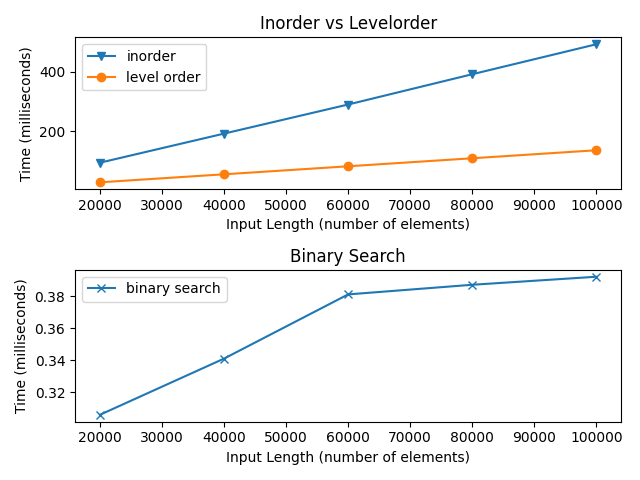
\includegraphics{1}

\subsection{Analysis}
\label{sec:analysis}
We know that for finding an element using level order traversal or inorder traversal, the time complexity is O(n) as every element in the array is accessed exactly once in the worst case. And the empirical results also prove this as we get a straight line in the graph. We also see that the slope of inorder traversal is greater than that of level order traversal. It is due to the fact that I have used recursion for inorder traversal where the function calls and the extra complexity due to this takes some extra constant time with each element access.\\

We also know that for finding an element using binary search from a sorted array, the time complexity is O(log(n)). This is also proved by empirical results as we can see that the increase in time taken for larger input size decreases as we increase the input size which is similar to the graph of log(n).\\

From this we can deduce that for faster searches, it is better to use binary search on a sorted array. And for unsorted array, level order traversal is empirically better than inorder traversal when stored using an array.\\

As for space, in case of levelorder and inorder, I am creating an array from input and storing the input data inside that. Hence the space complexity will be O(n). In case of binary search, I am setting the pointer to the input array and sorting the input array hence no extra space is required for the input. Hence the space complexity in this case is O(1).

\end{document}



%%% Local Variables:
%%% mode: latex
%%% TeX-master: t
%%% End:
